\documentclass[10pt,a4paper]{article}
\usepackage[a4paper,margin=1.85cm,top=1.7cm,bottom=1.7cm]{geometry}
\usepackage{amsmath,amssymb,bm}
\usepackage{booktabs}
\usepackage{graphicx}
\usepackage{subcaption}
\usepackage[font=small,labelfont=bf,skip=3pt]{caption}
\usepackage{listings}
\usepackage{xcolor}
\usepackage{enumitem}
\usepackage{microtype}
\usepackage{titlesec}
\usepackage[hidelinks]{hyperref}
\usepackage{array}
\usepackage{multirow}

\titleformat{\section}{\large\bfseries}{\thesection}{0.6em}{}
\titlespacing*{\section}{0pt}{9pt}{4pt}
\titleformat{\subsection}{\normalsize\bfseries}{\thesubsection}{0.5em}{}
\titlespacing*{\subsection}{0pt}{6pt}{2pt}
\titleformat{\subsubsection}[runin]{\bfseries}{}{0em}{}[.]
\titlespacing*{\subsubsection}{0pt}{4pt}{4pt}
\setlength{\parskip}{2.5pt}
\setlength{\emergencystretch}{1.5em}
\setlength{\parindent}{0pt}
\setlist{nosep,leftmargin=1.2em}
\setlength{\abovecaptionskip}{3pt}
\setlength{\textfloatsep}{8pt}
\setlength{\intextsep}{6pt}

\lstset{basicstyle=\ttfamily\scriptsize,columns=fullflexible,keepspaces=true,frame=single,framesep=2pt,
  rulecolor=\color{gray!60},backgroundcolor=\color{gray!5},xleftmargin=2pt,xrightmargin=2pt,breaklines=true,
  commentstyle=\color{gray!80},morecomment=[l]{//},aboveskip=3pt,belowskip=3pt}

\newcommand{\Rhat}{\widehat{R}}
\newcommand{\HDI}[2]{[#1,\,#2]}
\newcommand{\code}[1]{\texttt{#1}}

\begin{document}

\begin{center}
{\LARGE\bfseries CS702 Computational Interaction --- Group Assignment 1}\\[4pt]
{\large Bayesian hierarchical modelling $\cdot$ Simulating a conversational agent $\cdot$ Sequential decision making}\\[5pt]
{\textbf{Team members:} \textit{Name 1 (student ID), Name 2 (student ID), Name 3 (student ID)} \qquad AY2026--27 Term 1, Week 8}\\[3pt]
{\small All code (Python 3.12, NumPyro/ArviZ, PRISM 4.10, Pyomo/HiGHS) is in the accompanying archive; \code{README.md} lists how to run every script. All seeds are fixed.}
\end{center}
\vspace{-4pt}

% =====================================================================================================
\section{Problem 1: Bayesian hierarchical modelling of final mathematics grades}

\subsection{Q1.a Hypotheses and conceptual validation}
We model the final grade \code{G3} $\in\{0,\dots,20\}$ of the 395 students of the UCI mathematics data set without using the interim grades \code{G1}, \code{G2}. Two hypotheses lead to two structurally different generative stories.

\textbf{H1 (individual behaviour and background).} A student's final grade is explained by their own academic history and behaviour: past class failures and going out lower the grade; weekly study time, the wish to pursue higher education and the mother's education raise it; absences are expected to lower it. The effects are the same for every student, whichever school or family context they come from (\emph{complete pooling}). This is grounded in the original analysis of this data set, where past failures, absences and parental education were among the most informative attributes once \code{G1}/\code{G2} are removed \cite{cortez2008}, and in meta-analytic evidence that family socio-economic status is a robust correlate of achievement \cite{sirin2005}.

\textbf{H2 (contextual, group-level variation).} Beyond individual attributes, students are nested in social contexts, the school they attend (\code{school}: GP, $n{=}349$; MS, $n{=}46$) and the occupational background of the family (\code{Mjob}, five categories), and these contexts shift the expected grade of otherwise similar students. School-effects research finds between-school variation that is real but modest relative to family background \cite{coleman1966,raudenbush2002}, which motivates \emph{partial pooling}: group offsets are estimated, but shrunk towards a common mean by an amount learned from the data.

Both stories pass a face-validity check: they describe plausible mechanisms (prior achievement, effort, aspiration, family resources, school context), the predictors precede the outcome in time, and the predicted directions of effects agree with common sense. They differ in structure: H1 needs only student-level coefficients, H2 adds a hierarchy with group-level scales. Because Model~2 nests Model~1, comparing them isolates the predictive value of the context structure.

\subsection{Q1.b Model specification}
Let $x_i$ be the six standardised predictors (past failures, $\log(1+\text{absences})$, study time, going out, mother's education; \code{higher} is kept as 0/1). \textbf{Likelihood.} Both models use a Normal likelihood for \code{G3}: the bulk of the grades is roughly symmetric around the passing mark 10 (Fig.~\ref{fig:eda}a), and a continuous likelihood keeps the coefficients directly interpretable in grade points. The score is bounded and has a spike at 0, which a Normal cannot reproduce; we keep this as an explicit limitation to be tested by the predictive checks.

\textbf{Model 1 (H1, complete pooling).} $\;G3_i \sim \mathcal N(\mu_i,\sigma)$, $\mu_i=\alpha+x_i^{\top}\beta$, with $\alpha\sim\mathcal N(10,3)$, $\beta_k\sim\mathcal N(0,1)$, $\sigma\sim\text{HalfNormal}(5)$.

\textbf{Model 2 (H2, hierarchical, partial pooling).}
\begin{equation*}
\begin{aligned}
G3_i &\sim \mathcal N(\mu_i,\sigma),\qquad
\mu_i=\alpha + a_{\text{school}[i]} + b_{\text{Mjob}[i]} + x_i^{\top}\beta,\\
a_j &\sim\mathcal N(0,\sigma_{\text{sch}}),\qquad b_m\sim\mathcal N(0,\sigma_{\text{job}}),\qquad
\sigma_{\text{sch}},\sigma_{\text{job}}\sim\text{HalfNormal}(2),
\end{aligned}
\end{equation*}
with the same priors for $\alpha,\beta,\sigma$. The intercepts are partially pooled across the two schools and the five maternal-occupation groups: each group has its own offset, but the offsets are drawn from a common distribution whose scale ($\sigma_{\text{sch}}$, $\sigma_{\text{job}}$) is learned. Small groups (MS, $n{=}46$; \code{health}, $n{=}34$) are therefore shrunk towards the population, and if the data show no context effect the scales collapse towards zero and Model~2 reduces to Model~1. The code uses a non-centred parameterisation ($a_j=\sigma_{\text{sch}}z_j$) for sampling efficiency. The plate diagrams are shown in Fig.~\ref{fig:plates}: shaded nodes are observed, the dashed node $\mu_i$ is deterministic, and the plates show the student, school and \code{Mjob} replications with the arrows from the group offsets into every student's $\mu_i$.

\begin{figure}[t]
\centering
\begin{subfigure}[b]{0.30\textwidth}\centering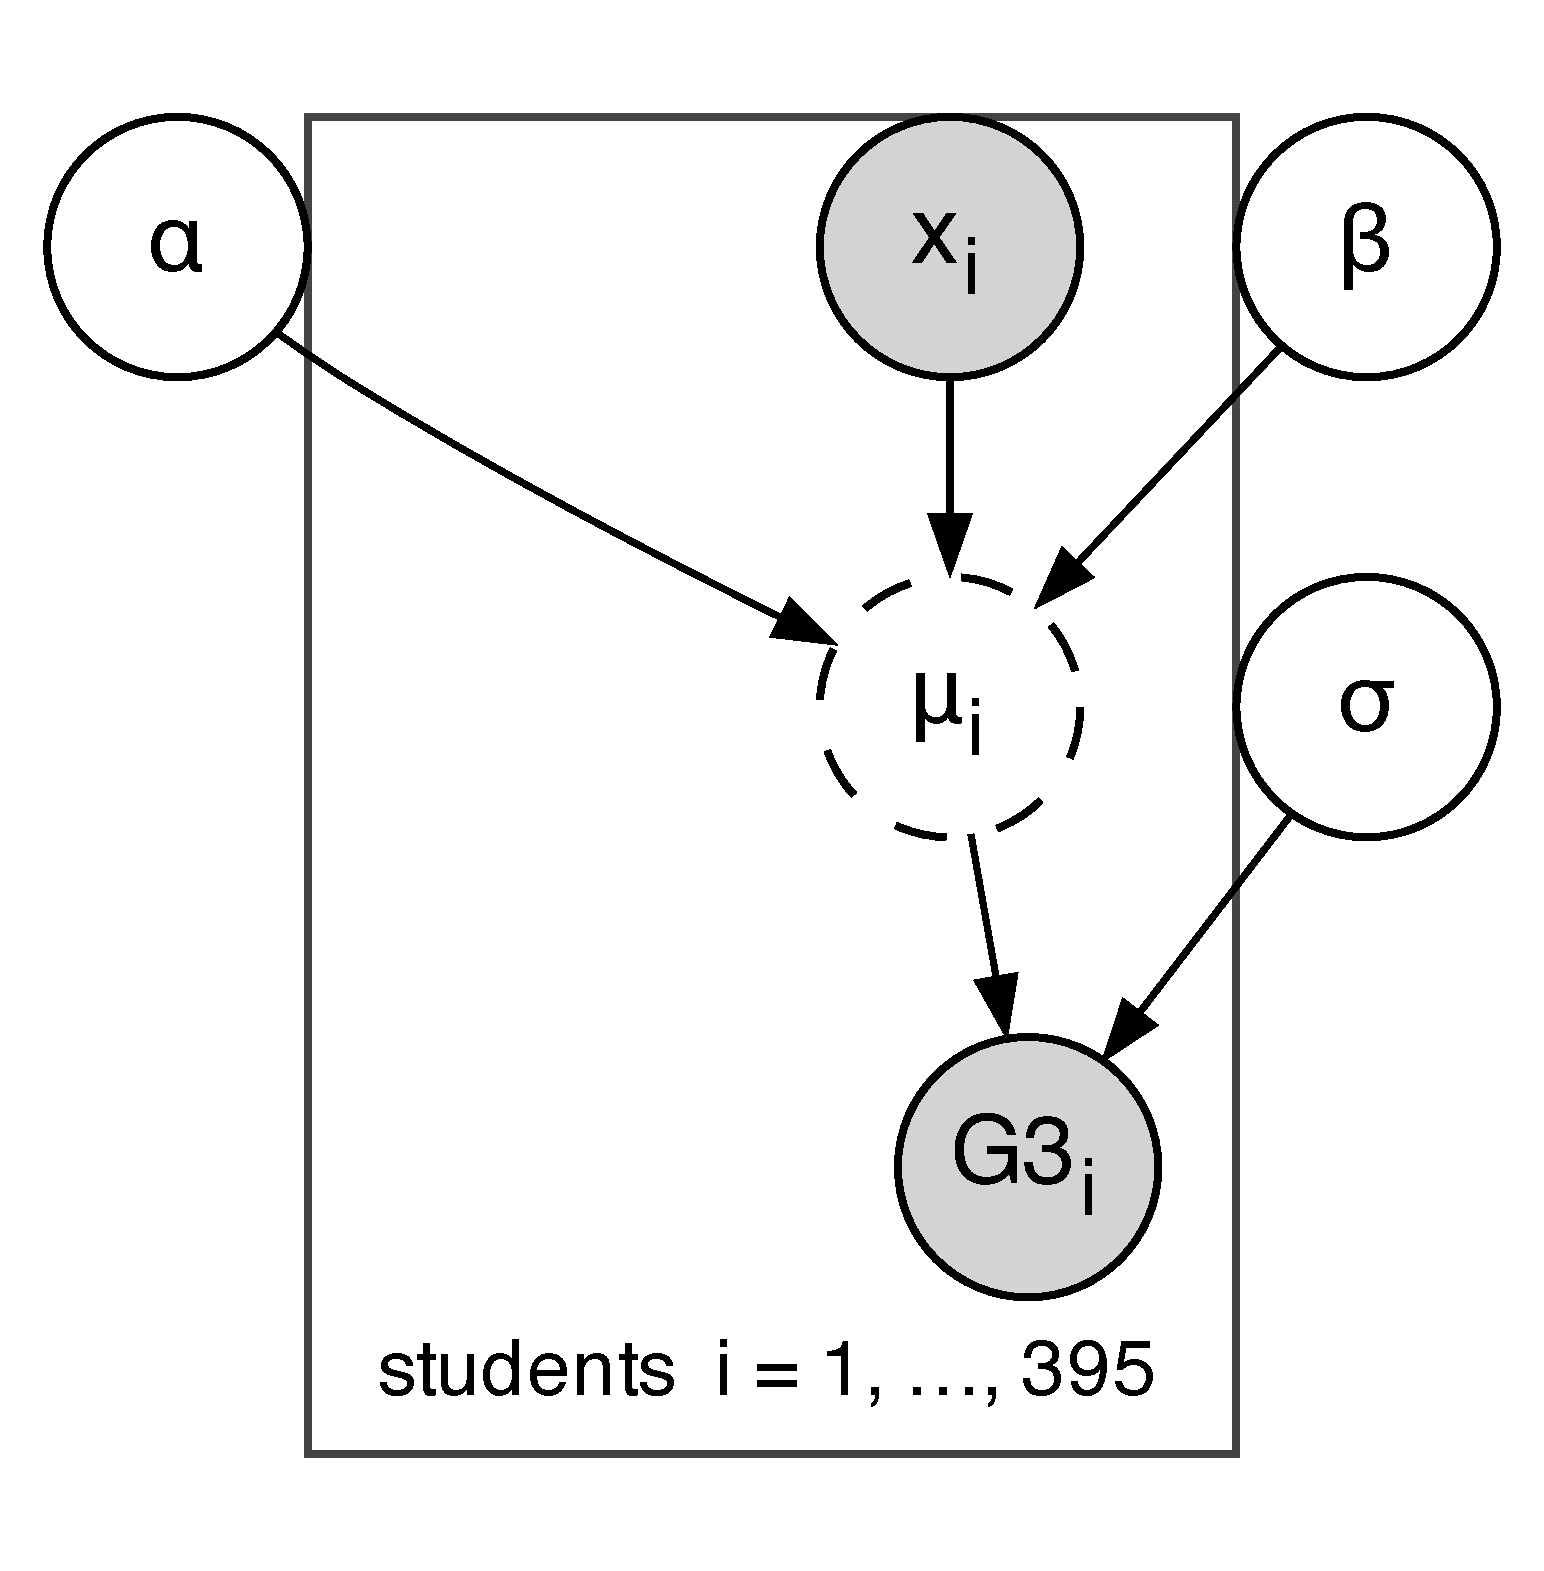
\includegraphics[height=3.4cm]{figures/plate_m1.pdf}\caption{Model 1 (complete pooling)}\end{subfigure}\hspace{1.2cm}
\begin{subfigure}[b]{0.55\textwidth}\centering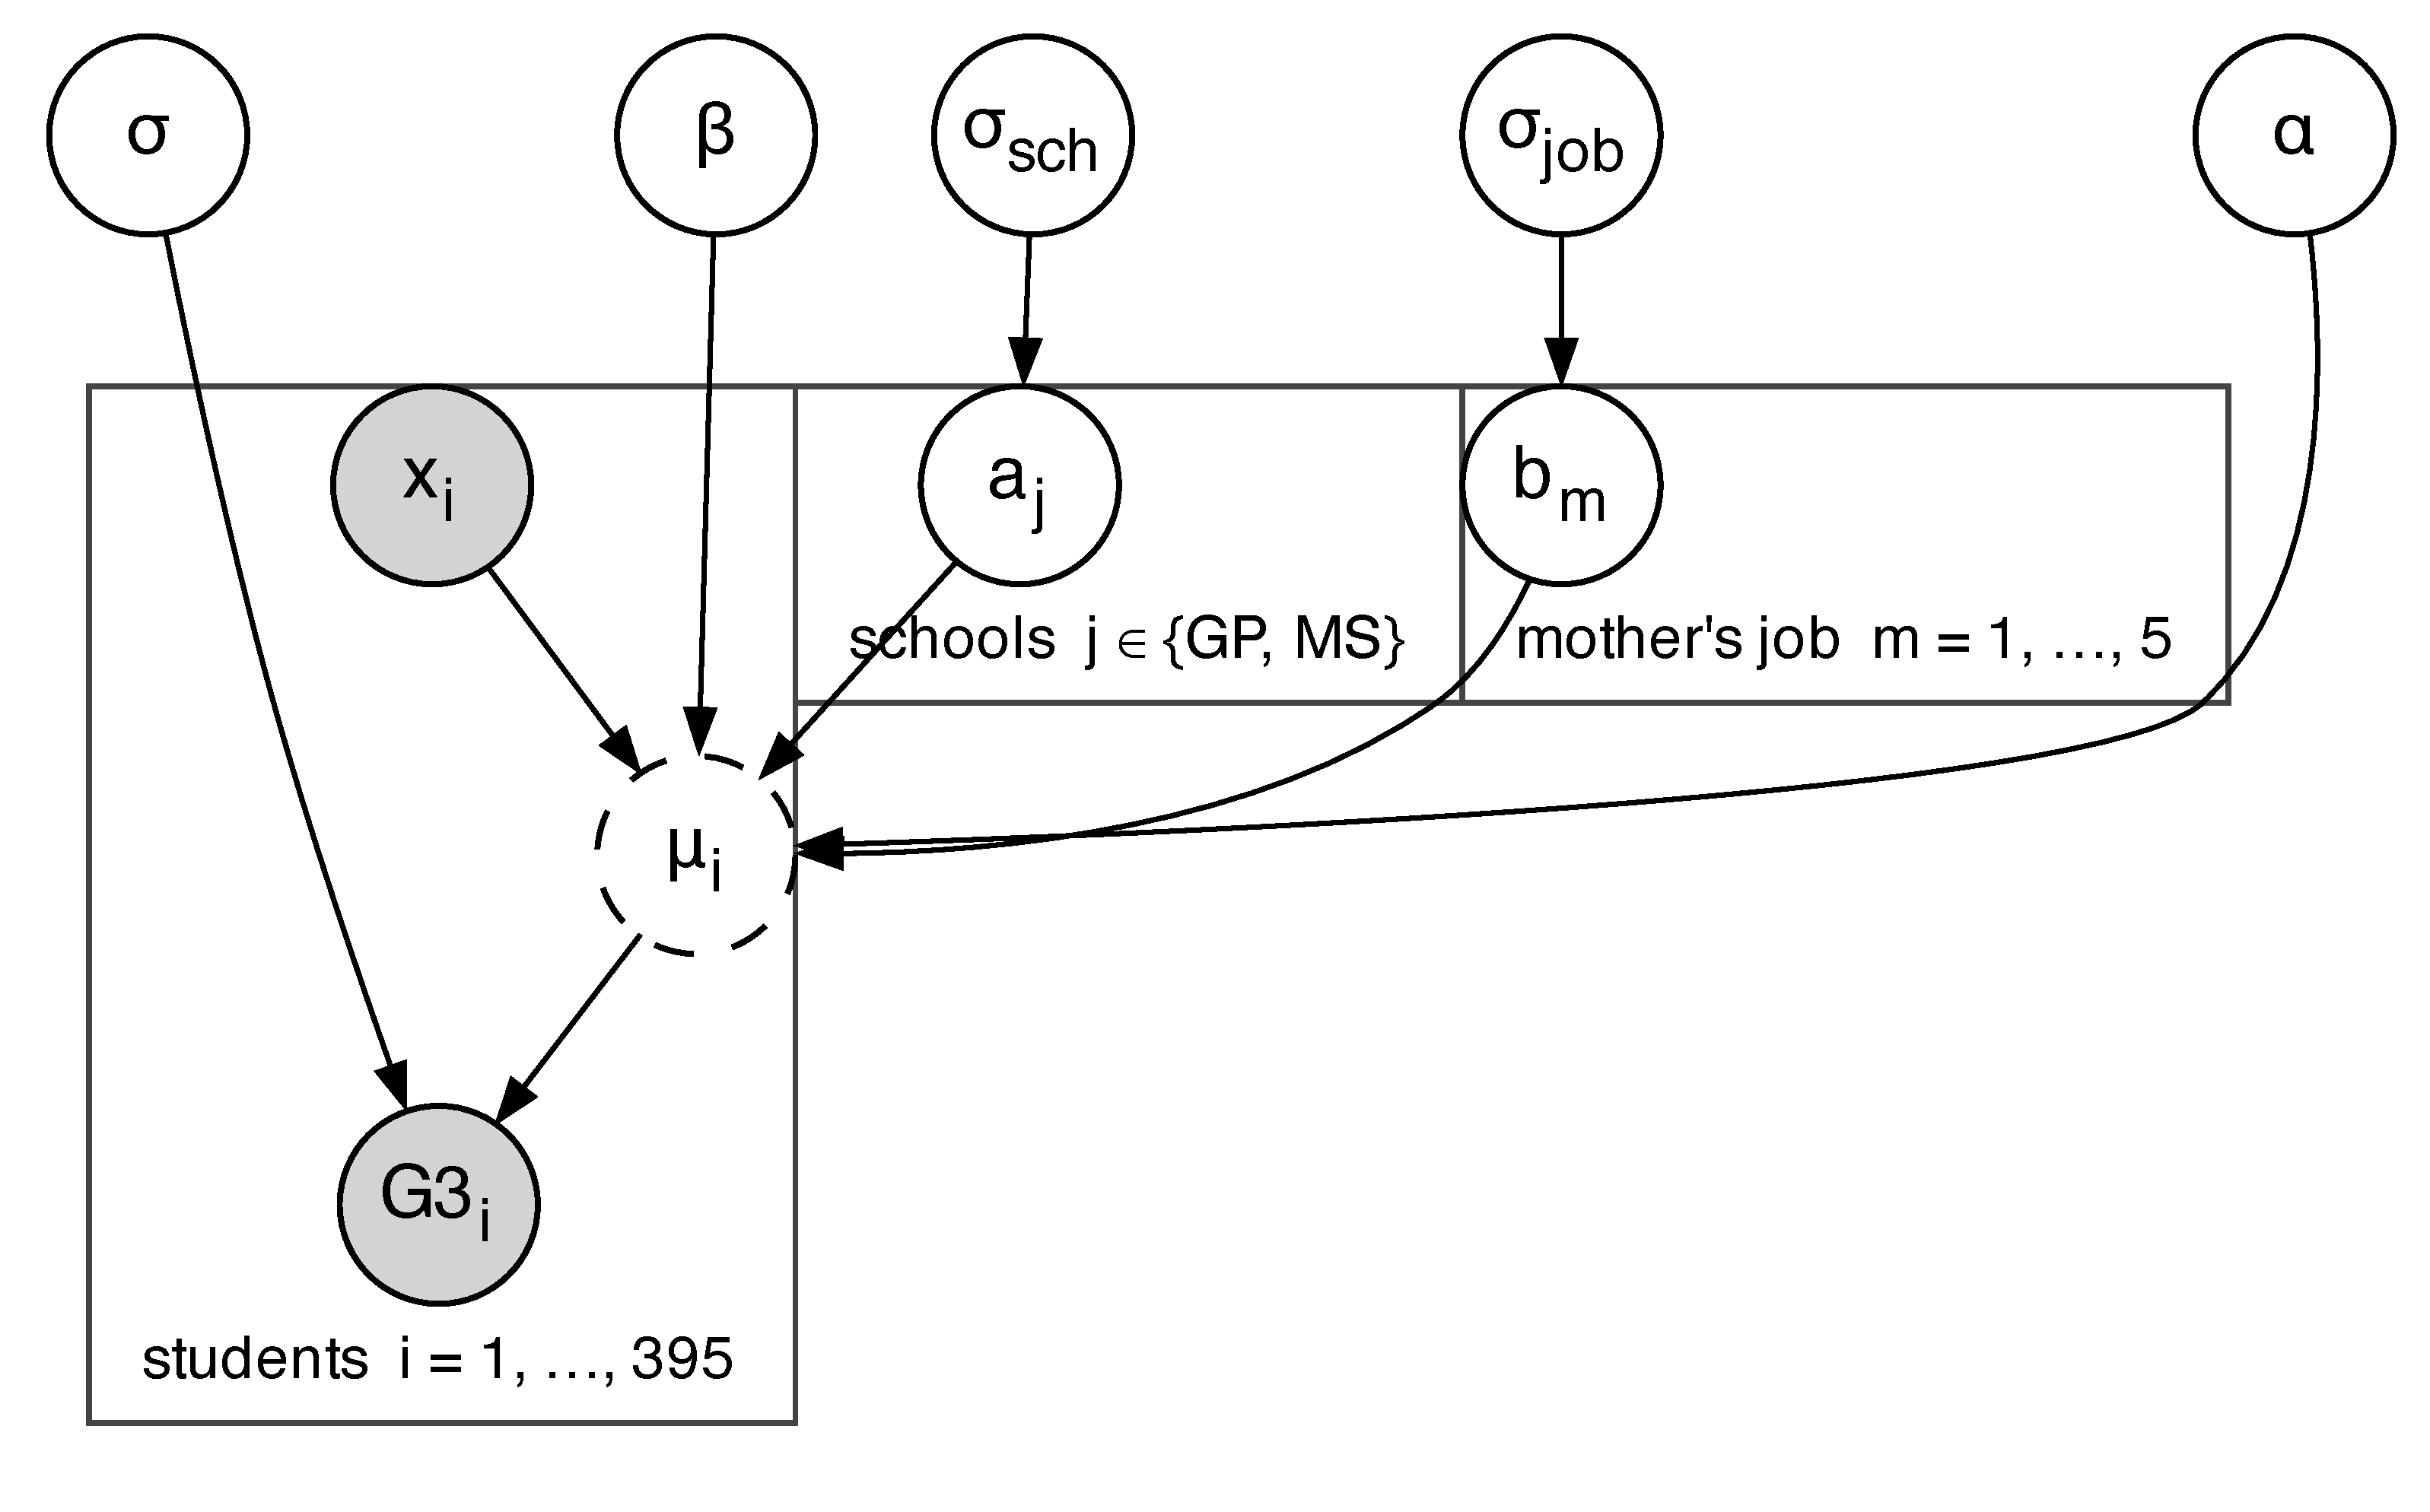
\includegraphics[height=3.4cm]{figures/plate_m2.pdf}\caption{Model 2 (varying intercepts by school and mother's job)}\end{subfigure}
\caption{Plate diagrams. $x_i$: standardised predictors; $\mu_i=\alpha+x_i^\top\beta$ (+ $a_j+b_m$ in Model 2); $G3_i\sim\mathcal N(\mu_i,\sigma)$.}
\label{fig:plates}
\end{figure}

\subsection{Q2 Prior predictive check and exploratory data analysis}
\subsubsection{Q2.a Initial parameters} Our first choice was deliberately vague: $\alpha\sim\mathcal N(0,10)$, $\beta_k\sim\mathcal N(0,5)$, $\sigma\sim\text{HalfNormal}(10)$, group scales $\text{HalfNormal}(10)$. The revised, weakly informative priors listed above encode what we know about a 0--20 grade scale without using the data: the average grade is around the passing mark ($\alpha\sim\mathcal N(10,3)$ puts 95\% of the baseline between 4 and 16); an effect larger than $\pm 2$--3 grade points per standard deviation of a predictor would be implausible ($\beta_k\sim\mathcal N(0,1)$); student-to-student spread of a few points ($\sigma\sim\text{HalfNormal}(5)$); context shifts of at most a few points ($\text{HalfNormal}(2)$). We have no domain knowledge about the \emph{sign} or size of individual effects, so the coefficient priors stay centred at zero and symmetric.

\subsubsection{Q2.b Prior predictive simulations} We drew 1000 parameter sets from each prior and simulated a full data set of 395 grades from each (Fig.~\ref{fig:prior}). Under the initial priors 63\% (Model 1) and 69\% (Model 2) of simulated grades fall outside 0--20, the 5--95\% range of a simulated grade is $-30$ to $30$ ($-39$ to $38$), and simulated data sets have standard deviations of 7--23 points: the priors describe impossible classrooms. Under the revised priors the 5--95\% range is $-0.3$ to $20.1$ (Model 1) and $-1.4$ to $20.9$ (Model 2), simulated class means span 4--16 and class standard deviations 2--10, i.e.\ the priors cover every plausible data set while remaining uninformative about which effects exist. \textbf{Revision:} we adopted the revised priors for all subsequent analyses; the remaining 10--13\% of simulated grades outside the scale is the price of an unbounded Normal likelihood, which we accept for the reasons given in Q1.b.

\begin{figure}[t]
\centering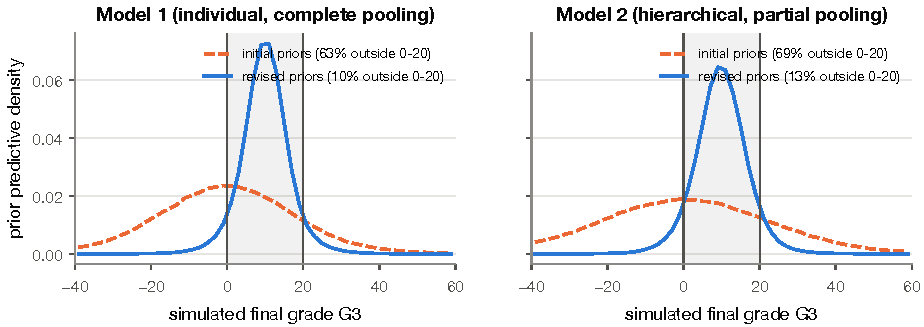
\includegraphics[width=\textwidth]{figures/fig_prior_predictive.pdf}
\caption{Prior predictive distributions of a simulated final grade under the initial (dashed) and revised (solid) priors; the grey band is the admissible 0--20 range.}
\label{fig:prior}
\end{figure}

\subsubsection{Q2.c EDA} The data set has 395 students and 33 attributes (30 predictors plus \code{G1}--\code{G3}). \code{G3} has mean 10.42, standard deviation 4.58, median 11 and range 0--20; 38 students (9.6\%) have \code{G3}${}=0$, a spike that is separated from the rest of the distribution (Fig.~\ref{fig:eda}a). These students have zero recorded absences (mean 0.0 versus 6.3 for the others) and \code{G2}${}=0$ in most cases, i.e.\ they left the course rather than failed an exam. The variables used in the models: past failures 0--3 (mean grade 11.3, 8.1, 6.2, 5.7 for 0, 1, 2, 3 failures; $r=-0.36$), absences 0--75 with a heavy right tail (hence the $\log(1+\cdot)$ transform; $r=0.03$), study time 1--4 (means 10.1, 10.2, 11.4, 11.3; $r=0.10$), \code{higher} (yes 10.6, no 6.8 for the 20 students who do not plan higher education), going out 1--5 ($r=-0.13$) and mother's education 0--4 ($r=0.22$). The grouping variables: GP ($n{=}349$, mean 10.5) versus MS ($n{=}46$, 9.9), and mother's job from 9.2 (\code{at\_home}, $n{=}59$) to 12.2 (\code{health}, $n{=}34$) (Fig.~\ref{fig:eda}b,c). These facts support the modelling choices: a symmetric bulk (Normal likelihood), monotone predictor effects that can be captured by linear terms, group differences of 1--3 points that are small relative to the within-group spread (partial pooling rather than separate models), and a warning that the zero spike, which is not related to absences, will be misfit.

\begin{figure}[t]
\centering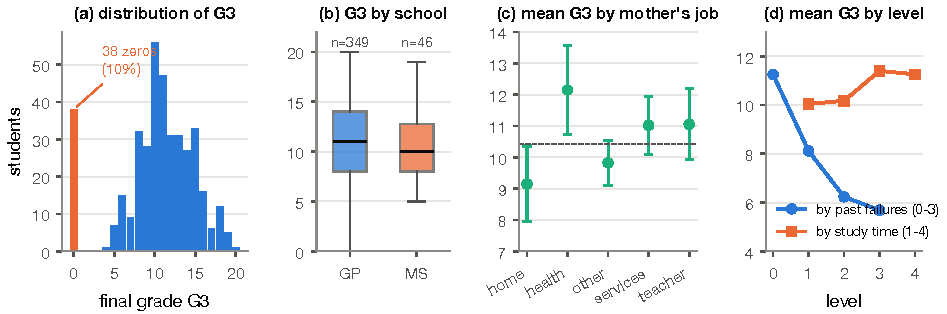
\includegraphics[width=\textwidth]{figures/fig_eda.pdf}
\caption{EDA: (a) the distribution of \code{G3} with the 38 zeros highlighted; (b) grades by school; (c) mean grade by mother's job with 95\% confidence intervals (dashed: overall mean); (d) mean grade by number of past failures and by weekly study time.}
\label{fig:eda}
\end{figure}

\subsection{Q3 Posterior inference and model comparison}
\subsubsection{Q3.a Posterior inference} Both models were fitted with NUTS in NumPyro (4 chains, 1000 warm-up and 1500 retained draws each, target acceptance 0.99). Convergence is unproblematic: Model 1 $\Rhat_{\max}=1.001$, minimum bulk ESS 3396; Model 2 $\Rhat_{\max}=1.004$, minimum ESS 1596; no divergent transitions. Table~\ref{tab:post} reports the posterior means and 95\% HDIs, and Fig.~\ref{fig:post} shows them graphically.

\begin{table}[t]
\centering\footnotesize
\caption{Posterior mean and 95\% HDI of the key parameters. Coefficients are grade points per one standard deviation of the predictor (\code{higher}: yes versus no).}
\label{tab:post}
\setlength{\tabcolsep}{3pt}
\begin{tabular}{lcc@{\hspace{10pt}}lc}
\toprule
Parameter & Model 1 & Model 2 & Model 2 only & \\
\midrule
$\alpha$ (baseline grade) & 9.83 \HDI{8.52}{11.18} & 9.97 \HDI{7.92}{12.25} & $\sigma_{\text{sch}}$ (between-school sd) & 0.90 \HDI{0.00}{2.71}\\
past failures & $-1.35$ \HDI{-1.77}{-0.92} & $-1.40$ \HDI{-1.81}{-0.96} & $\sigma_{\text{job}}$ (between-Mjob sd) & 0.89 \HDI{0.00}{1.93}\\
absences ($\log(1+\cdot)$) & 0.78 \HDI{0.37}{1.18} & 0.79 \HDI{0.39}{1.20} & $a_{\text{GP}}$ / $a_{\text{MS}}$ & $-0.03$ \HDI{-1.70}{1.78} / 0.06 \HDI{-1.63}{1.87}\\
weekly study time & 0.15 \HDI{-0.25}{0.55} & 0.16 \HDI{-0.26}{0.56} & $b_{\text{at\_home}}$ & $-0.43$ \HDI{-1.85}{0.69}\\
wants higher education & 0.61 \HDI{-0.75}{1.94} & 0.56 \HDI{-0.81}{1.95} & $b_{\text{health}}$ & 0.65 \HDI{-0.52}{2.18}\\
going out & $-0.53$ \HDI{-0.94}{-0.13} & $-0.55$ \HDI{-0.98}{-0.17} & $b_{\text{other}}$ & $-0.36$ \HDI{-1.56}{0.72}\\
mother's education & 0.58 \HDI{0.14}{0.96} & 0.47 \HDI{-0.01}{0.96} & $b_{\text{services}}$ & 0.50 \HDI{-0.60}{1.68}\\
$\sigma$ (residual sd) & 4.15 \HDI{3.88}{4.46} & 4.13 \HDI{3.84}{4.41} & $b_{\text{teacher}}$ & $-0.33$ \HDI{-1.65}{0.86}\\
\bottomrule
\end{tabular}
\end{table}

\begin{figure}[t]
\centering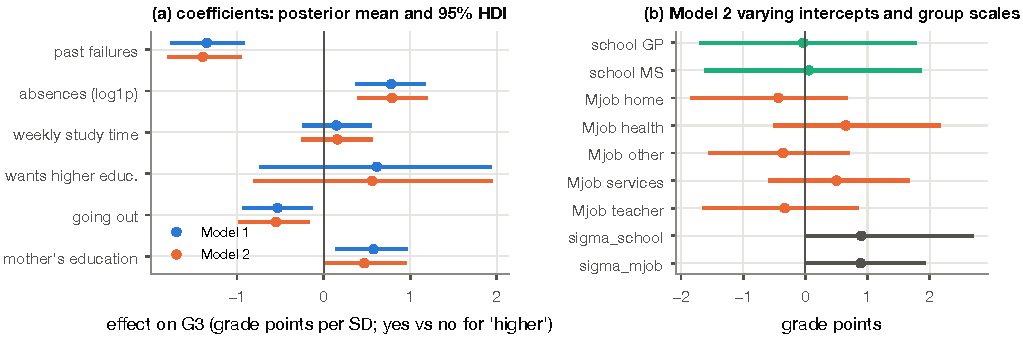
\includegraphics[width=\textwidth]{figures/fig_posterior.pdf}
\caption{Posterior means and 95\% HDIs: (a) predictor coefficients of both models; (b) the varying intercepts and group scales of Model 2.}
\label{fig:post}
\end{figure}

\emph{Are the estimates sensible?} Past failures have the largest effect: $-1.35$ points per standard deviation (0.74 failures), i.e.\ about $-1.8$ points per additional failed year, matching the EDA gradient. Going out ($-0.53$) and mother's education ($+0.58$) have the expected signs with HDIs excluding zero; the study-time effect is small and uncertain ($+0.15$, HDI covering zero), and the wish for higher education is positive but poorly determined because only 20 students answered ``no''. One coefficient contradicts H1: absences have a \emph{positive} effect ($+0.78$ per SD). This is the data artefact identified in the EDA: the 38 zero-grade students all have zero recorded absences, so within a Normal model ``no absences'' is associated with the lowest grades. The model has no component for course withdrawal, and the coefficient absorbs it. In Model 2 the mother's-education coefficient shrinks from 0.58 to 0.47 because the \code{Mjob} offsets absorb part of the family-background signal, and its HDI now touches zero. The school offsets are essentially zero ($-0.03$ and $+0.06$) with a between-school scale that is indistinguishable from its prior (with only two schools $\sigma_{\text{sch}}$ is barely identified); the \code{Mjob} offsets are ordered as in the EDA (\code{health} $+0.65$, \code{services} $+0.50$, \code{at\_home} $-0.43$) but shrunk to roughly a third of the raw group differences and all HDIs include zero. Partial pooling behaves as intended: the raw \code{health} advantage of $+1.7$ points ($n{=}34$) is pulled towards the population once the individual predictors are accounted for.

\begin{figure}[t]
\centering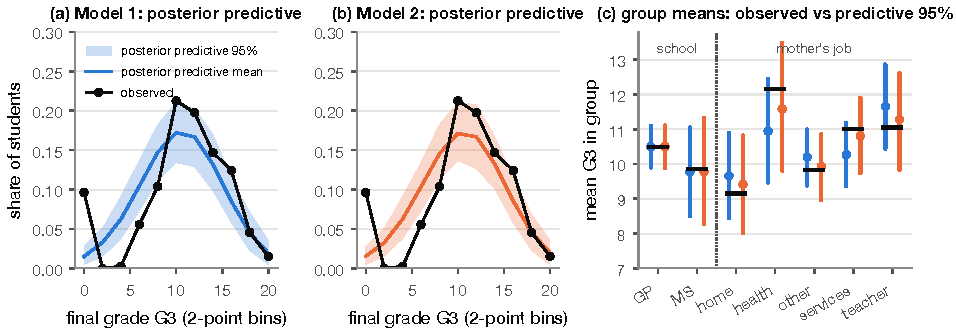
\includegraphics[width=\textwidth]{figures/fig_ppc.pdf}
\caption{Posterior predictive checks. (a,b) Share of students per 2-point grade bin: observed (black) versus the posterior predictive mean and 95\% interval. (c) Mean grade per group: observed (black bar) versus the posterior predictive 95\% intervals of Model 1 (blue) and Model 2 (orange).}
\label{fig:ppc}
\end{figure}

\emph{Posterior predictive checks} (Fig.~\ref{fig:ppc}). Both models reproduce the overall mean (observed 10.42; predictive 10.41 \HDI{9.84}{10.99}) and standard deviation (4.58; predictive 4.60 \HDI{4.17}{5.06}), the shape of the distribution between 6 and 20, and the group means: all seven observed group means lie inside the predictive 95\% intervals of both models (panel c), with Model 2 tracking the \code{Mjob} means more closely (\code{health}: observed 12.15, Model 1 predicts 10.94, Model 2 11.58). Where the models fall short is exactly where the EDA predicted: the zero spike (observed 9.6\% of students, predicted 1.9\% \HDI{0.8\%}{3.5\%}, Bayesian $p<0.001$), the empty region between 1 and 4 (predicted 3--6\% of students per 2-point bin), and the bounds (1.5\% of predicted grades are below 0 and 1.6\% above 20; predicted minimum $-4.3$ and maximum $23.6$ against the observed 0 and 20). The in-sample RMSE of the posterior predictive mean is 4.11 (Model 1) and 4.07 (Model 2) against a raw standard deviation of 4.58, i.e.\ the six predictors explain about 20\% of the variance of \code{G3}, which is what one expects when the interim grades are excluded.

\subsubsection{Q3.b Model comparison with LOO} PSIS-LOO (ArviZ) gives $\text{elpd}_{\text{loo}}=-1125.7$ (SE 14.7, $p_{\text{loo}}=11.5$) for Model 2 and $-1126.4$ (SE 14.4, $p_{\text{loo}}=7.8$) for Model 1; all Pareto-$k$ diagnostics are below 0.35, so the estimates are reliable. The difference, $\Delta\text{elpd}=0.7$ with a standard error of 2.1, is far below the usual threshold of 4 and smaller than its own uncertainty; the stacking weights are 0.67 (Model 2) and 0.33 (Model 1). \textbf{Conclusion:} the two models predict new students equally well; the hierarchical model is nominally better but the difference is small and uncertain. The context structure of H2 therefore adds no measurable predictive value once the individual predictors of H1 are included, which is consistent with the literature that family background dominates school membership \cite{coleman1966}. The extra structure is also cheap: shrinkage keeps the effective number of parameters of Model 2 at 11.5 versus 7.8. Two qualifications about available data: (i) if student-level covariates were unavailable at prediction time, a purely group-based model would still carry information (\code{Mjob} group means differ by up to 3 points), and Model 2 would then be the only usable one; (ii) predictions for a \emph{new} school would rely on $\sigma_{\text{sch}}$, which two schools cannot pin down. Finally, both models share the same misspecification of the zero-grade process, so LOO ranks them on the 90\% of students they can describe; the natural next iteration of the workflow is a two-part (hurdle) likelihood with a Bernoulli component for course withdrawal, which would also remove the spurious positive absence effect.

\clearpage
% =====================================================================================================
\section{Problem 2: Simulating the HealthLine conversational agent}

\subsection{Q1.a MDP diagram}
Figure~\ref{fig:mdp} draws the twelve states $s_0,\dots,s_{11}$ (terminal states $s_7$--$s_{11}$ as double circles, $s_0$ with an incoming arrow). Each black square is the branching point of one action: the edge into the square carries the action name and the edges out of it the transition probabilities. The two actions with a certain outcome (\code{emergency\_referral} from $s_4$ and \code{offer\_nurse} from $s_5$) are drawn as single labelled edges. States $s_1$--$s_4$ each offer two actions and are the decision points of the system.

\begin{figure}[!htb]
\centering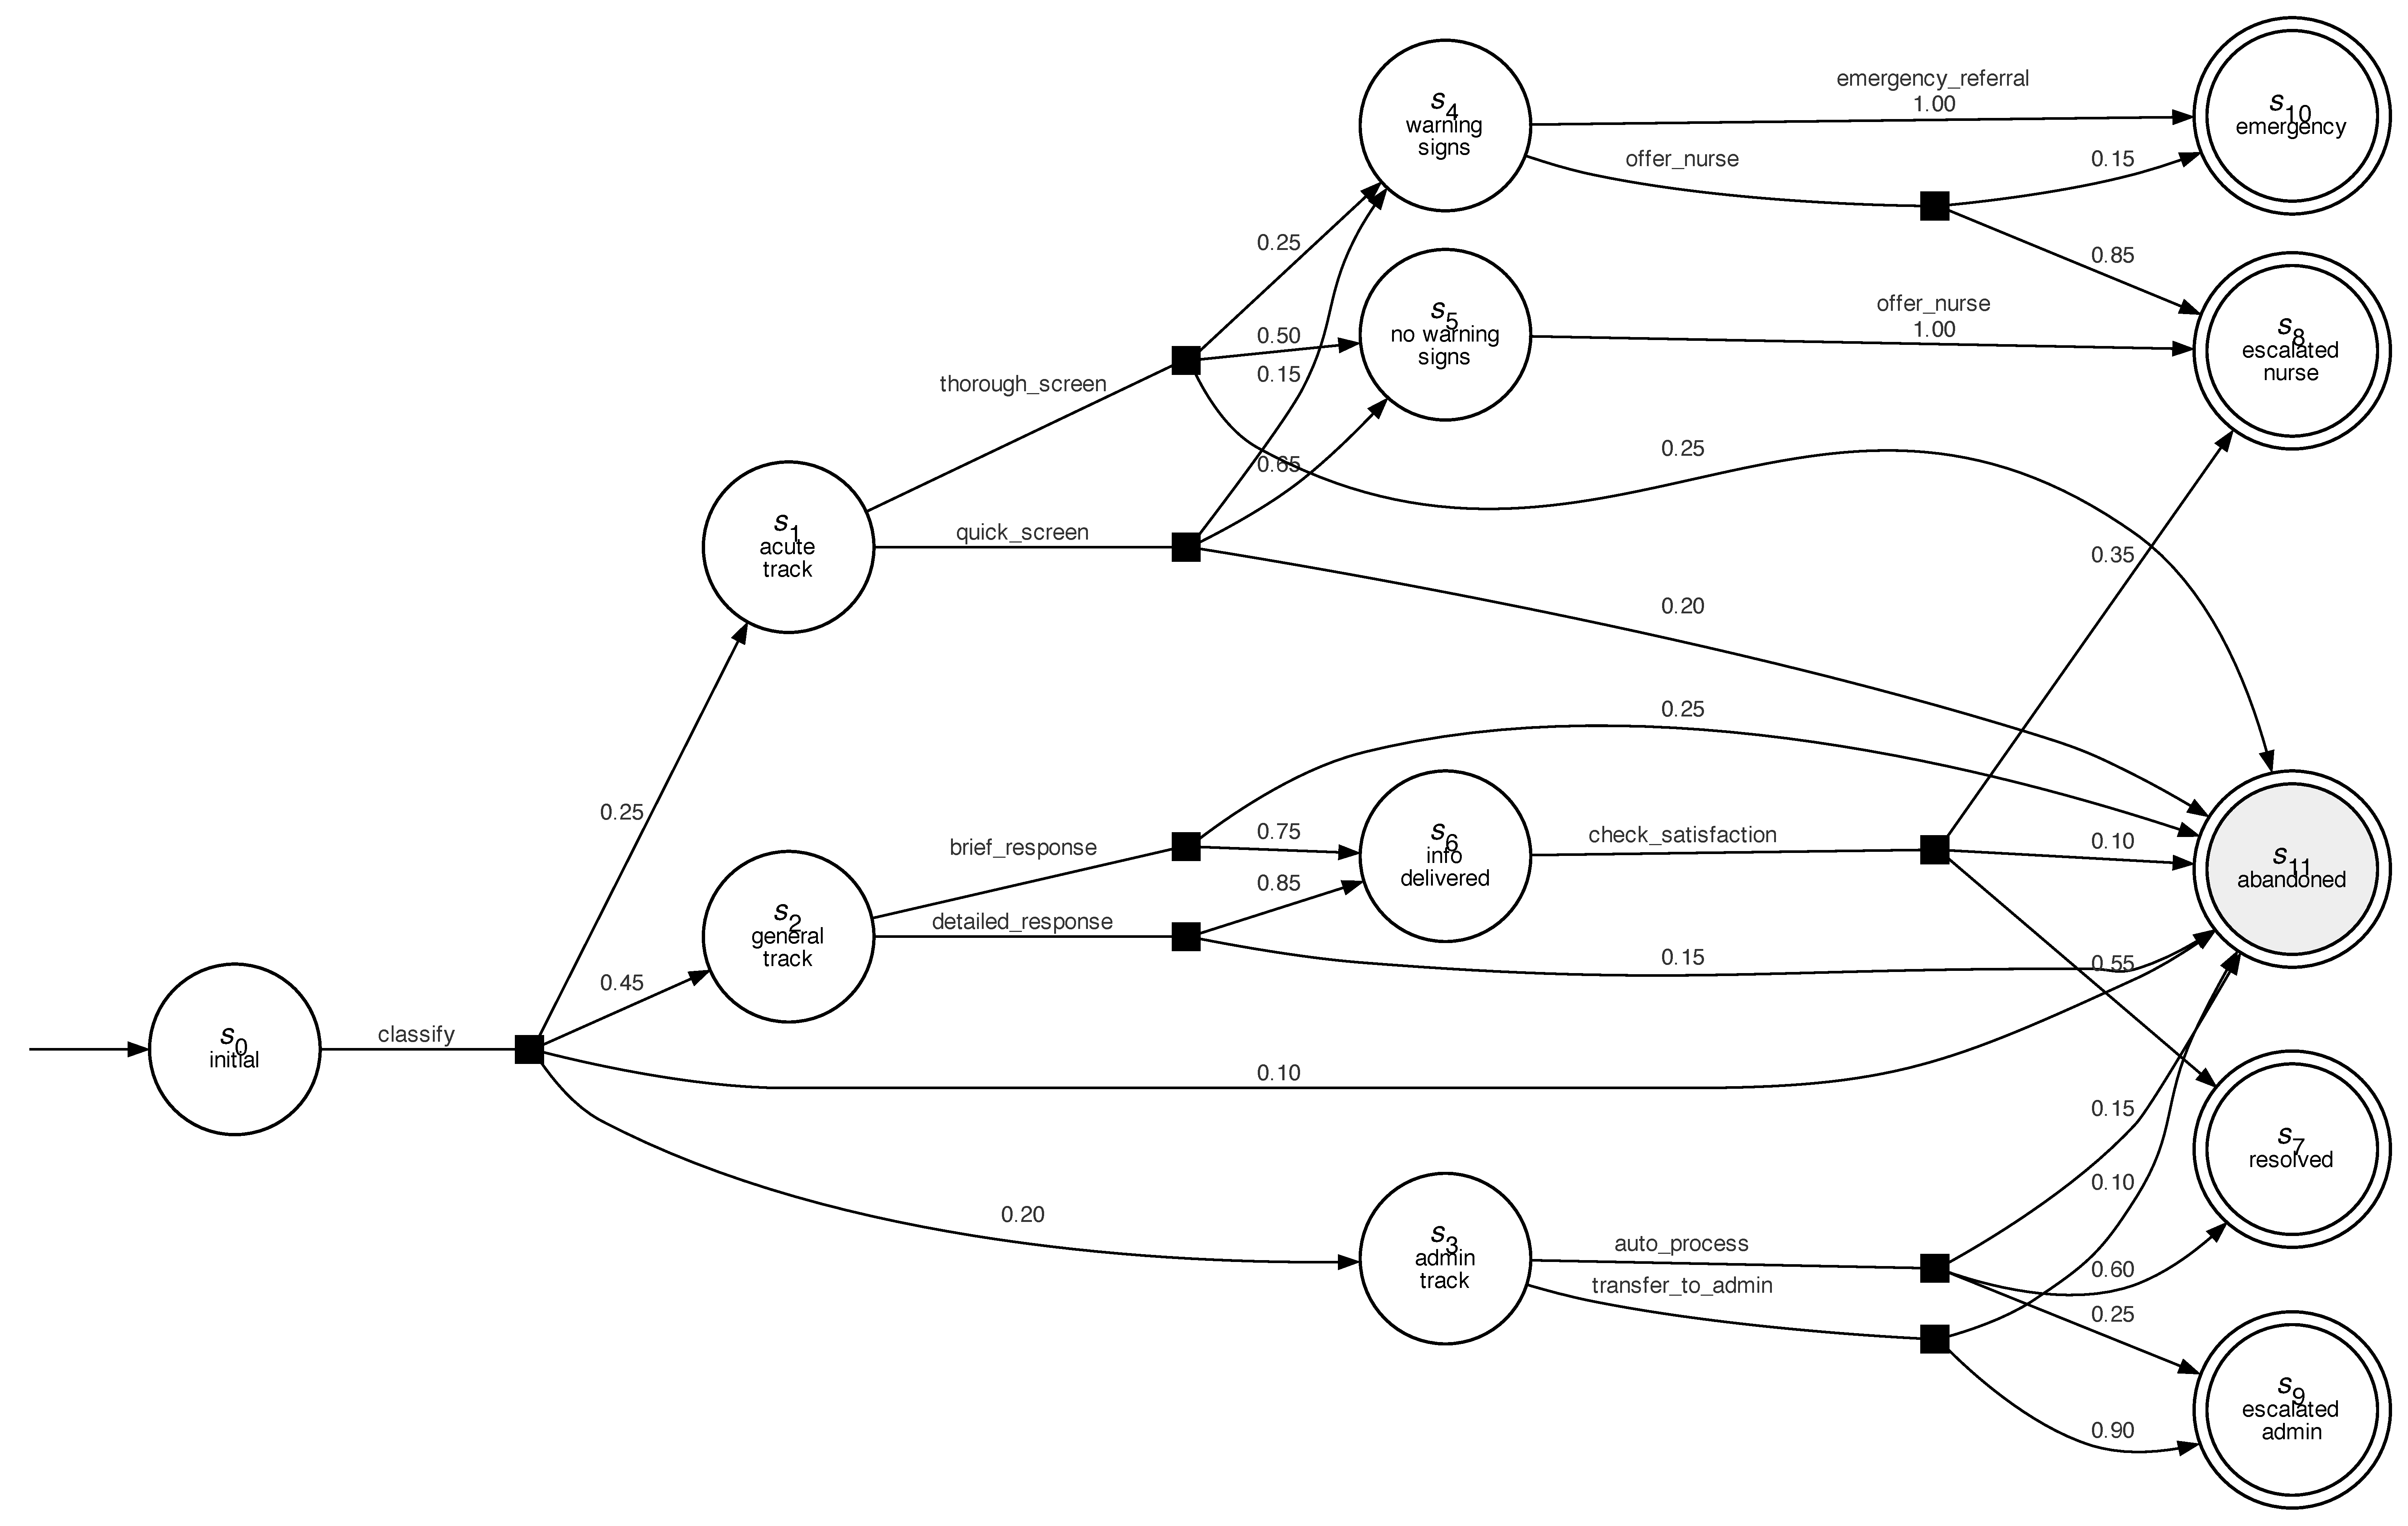
\includegraphics[width=0.96\textwidth]{figures/fig_mdp.pdf}
\caption{The HealthLine MDP. Circles: states; double circles: terminal states; black squares: probabilistic branching points of the actions; edge labels: action names and transition probabilities.}
\label{fig:mdp}
\end{figure}

\subsection{Q1.b PRISM model}
\code{healthline.pm} encodes the state as one bounded integer \code{s} and each (state, action) pair as one guarded command whose label is the action name. Terminal states carry a self-loop so that the model has no deadlocks, and a label per state name plus \code{"terminal"} for $s_7$--$s_{11}$. The rewards of the table are attached to the terminal states in the reward structure \code{"outcome"}. \code{prism healthline.pm} builds the model without errors and reports \textbf{12 states (1 initial) and 31 transitions}; the module has 16 commands (11 actions plus the 5 terminal self-loops).
\begin{lstlisting}
mdp
module healthline
    s : [0..11] init 0;   // 0 initial, 1 acute, 2 general, 3 admin, 4 warning signs, 5 no warning signs,
                          // 6 information delivered, 7 resolved, 8 esc. nurse, 9 esc. admin, 10 emergency, 11 abandoned
    [classify]           s=0 -> 0.25 : (s'=1) + 0.45 : (s'=2) + 0.20 : (s'=3) + 0.10 : (s'=11);
    [quick_screen]       s=1 -> 0.15 : (s'=4) + 0.65 : (s'=5) + 0.20 : (s'=11);
    [thorough_screen]    s=1 -> 0.25 : (s'=4) + 0.50 : (s'=5) + 0.25 : (s'=11);
    [brief_response]     s=2 -> 0.75 : (s'=6) + 0.25 : (s'=11);
    [detailed_response]  s=2 -> 0.85 : (s'=6) + 0.15 : (s'=11);
    [auto_process]       s=3 -> 0.60 : (s'=7) + 0.25 : (s'=9) + 0.15 : (s'=11);
    [transfer_to_admin]  s=3 -> 0.90 : (s'=9) + 0.10 : (s'=11);
    [emergency_referral] s=4 -> 1.00 : (s'=10);
    [offer_nurse]        s=4 -> 0.85 : (s'=8) + 0.15 : (s'=10);
    [offer_nurse]        s=5 -> 1.00 : (s'=8);
    [check_satisfaction] s=6 -> 0.55 : (s'=7) + 0.35 : (s'=8) + 0.10 : (s'=11);
    [done]               s>=7 -> true;          // terminal states are absorbing
endmodule
label "initial" = (s=0);  label "acute_track" = (s=1);  ...  label "resolved" = (s=7);  label "escalated_nurse" = (s=8);
label "escalated_admin" = (s=9);  label "emergency" = (s=10);  label "abandoned" = (s=11);  label "terminal" = (s>=7);
rewards "outcome"
    s=7 : 10;   s=8 : 6;   s=9 : 5;   s=10 : 12;   s=11 : 0;
endrewards
\end{lstlisting}

\subsection{Q1.c Forward simulation}
We generated 100 traces with PRISM's simulator (\code{prism healthline.pm -simpath 20 <file>}, once per trace). PRISM resolves the nondeterministic choice in $s_1$--$s_4$ uniformly at random and stops a path when the terminal self-loop is detected, so every trace runs from $s_0$ to a terminal state. Table~\ref{tab:sim} and Fig.~\ref{fig:sim} summarise the traces; the exact outcome distribution of the same uniform-random policy, computed from the transition matrix, is shown for comparison.
\begin{itemize}
\item \textbf{Most common outcomes.} Escalation to a nurse (37 traces) is the most common outcome, followed by abandonment (28) and resolution without escalation (23). The nurse outcome is frequent because every acute-track conversation without warning signs ends there and 35\% of the general-track conversations do too.
\item \textbf{Abandonment.} 28 of 100 traces ended in \code{abandoned} (Wilson 95\% interval 20--37\%), in line with the exact value 30.7\% for random choices; a tenth of all conversations are already lost at the classification step.
\item \textbf{Average reward.} The mean terminal reward is $5.47$ (standard error 0.39; exact expectation 5.25 under random choices). Traces are short: mean 2.6 transitions (67 traces need three, 26 two, 7 one).
\end{itemize}

\begin{table}[t]
\centering\small
\caption{Outcomes of the 100 simulated traces and the exact probabilities under the uniform-random resolution of the choices.}
\label{tab:sim}
\begin{tabular}{lccccc|cc}
\toprule
 & resolved & esc.\ nurse & esc.\ admin & emergency & abandoned & mean reward & mean length\\
\midrule
simulated traces & 23 & 37 & 7 & 5 & 28 & 5.47 $\pm$ 0.39 & 2.60\\
exact (random policy) & 25.8\% & 29.1\% & 11.5\% & 2.9\% & 30.7\% & 5.25 & 2.45\\
\bottomrule
\end{tabular}
\end{table}

\begin{figure}[t]
\centering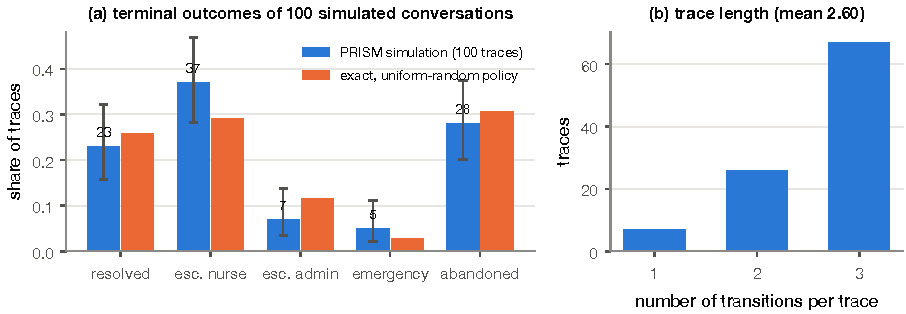
\includegraphics[width=0.9\textwidth]{figures/fig_simulation.pdf}
\caption{(a) Terminal outcomes of the 100 PRISM traces (bars with Wilson 95\% intervals) against the exact distribution under random choices; (b) number of transitions per trace.}
\label{fig:sim}
\end{figure}

\subsection{Q1.d Verification with PCTL}
Table~\ref{tab:pctl} lists the properties (file \code{healthline.props}), PRISM's results, and their meaning. Because the model is an MDP, PRISM quantifies over all policies (\code{Pmax}/\code{Pmin}). For the expected reward we use the instantaneous-reward operator: every episode is absorbed in a terminal state within three transitions, so the expected reward of the state occupied at step 3 (or any later step; \code{I=10} gives the same value) equals the expected terminal reward. The reachability form \code{R[F "terminal"]} would return 0, because PRISM excludes the reward of the target state itself. All values were reproduced by an independent value-iteration computation in Python (\code{p2\_verify.py}).

\begin{table}[t]
\centering\footnotesize
\caption{PCTL properties of the HealthLine MDP and their results.}
\label{tab:pctl}
\setlength{\tabcolsep}{4pt}
\begin{tabular}{>{\raggedright\arraybackslash}p{2.2cm}>{\raggedright\arraybackslash}p{5.0cm}c>{\raggedright\arraybackslash}p{7.6cm}}
\toprule
Question & PRISM property & Result & What it reveals\\
\midrule
Max.\ self-resolution & \code{Pmax=? [ F "resolved" ]} & 0.3304 & Even the best policy resolves at most a third of conversations without a human: \code{resolved} is reachable only via the general track ($0.45\cdot0.85\cdot0.55$) and the admin track ($0.20\cdot0.60$). (\code{Pmin} $=0.1856$ with brief responses and admin transfer.)\\
Abandonment & \code{Pmax=? [ F "abandoned" ]} & 0.3388 & Worst policy (thorough screening, brief responses, automatic processing).\\
 & \code{Pmin=? [ F "abandoned" ]} & 0.2758 & Best policy (quick screening, detailed responses, admin transfer). Abandonment stays between 27.6\% and 33.9\% whatever the policy; the 10\% lost at classification and the drop-off after each step are structural.\\
Overall success & \code{Pmax=? [ F ("terminal" \& !"abandoned") ]} & 0.7243 & Complement of the minimum abandonment: at most 72.4\% of patients reach a proper outcome (resolution, appropriate escalation or emergency care); \code{Pmin} $=0.6613$.\\
Expected reward & \code{R\{"outcome"\}max=? [ I=3 ]} & 5.857 & Best achievable expected outcome value per conversation.\\
 & \code{R\{"outcome"\}min=? [ I=3 ]} & 4.646 & Worst policy. The policy moves the expected value by 1.2 points ($\approx 26\%$), so policy design matters more for the outcome value than for abandonment.\\
\bottomrule
\end{tabular}
\end{table}

\subsection{Q2.a Linear program for the optimal policy}
Following the lecture note, we treat the state values $v(s)$ as decision variables and impose the Bellman optimality constraints. With $T=\{s_7,\dots,s_{11}\}$ the terminal states, $A(s)$ the actions of state $s$, $P(s'\mid s,a)$ the transition probabilities and $R(s')$ the reward collected on entering $s'$ (10, 6, 5, 12, 0 for $s_7,\dots,s_{11}$, and 0 otherwise):
\begin{equation*}
\min_{v}\;\sum_{s\in S\setminus T} v(s)
\quad\text{s.t.}\quad
v(s)\;\ge\;\sum_{s'} P(s'\mid s,a)\,\big[R(s')+\gamma\,v(s')\big]\;\;\forall s\in S\setminus T,\;a\in A(s);\qquad v(s)=0\;\;\forall s\in T .
\end{equation*}
There are 12 variables (7 free, 5 fixed to zero) and 11 constraints, one per (state, action) pair. Every feasible $v$ is an upper bound on the optimal values; minimising the sum pushes each $v(s)$ down until the constraint of the best action becomes tight, so the solution is the optimal value function and the total reward from $s_0$ is $v^\ast(s_0)$. Because every conversation ends after at most three transitions, the total reward is finite without discounting and we use $\gamma=1$ (the objective is then exactly the expected total reward). The optimal policy is read off as $\pi^\ast(s)=\arg\max_{a\in A(s)}\sum_{s'}P(s'\mid s,a)[R(s')+v^\ast(s')]$.

\subsection{Q2.b Implementation and solution}
The LP was implemented in Pyomo and solved with HiGHS (\code{p2\_lp\_policy.py}; status \emph{optimal}). Table~\ref{tab:lp} gives the state-action values $Q(s,a)$ and the optimal policy for the four states with a choice. The optimal expected total reward is $v^\ast(s_0)=5.857$, identical to PRISM's \code{Rmax}; re-solving the LP with reversed inequalities and a maximised objective gives the worst-case value 4.646, identical to \code{Rmin}, which confirms the formulation.

\begin{table}[t]
\centering\footnotesize
\caption{LP solution: state-action values and optimal actions in the decision states ($\gamma=1$). Non-decision states: $v^\ast(s_0)=5.857$, $v^\ast(s_5)=6.0$, $v^\ast(s_6)=7.6$.}
\label{tab:lp}
\setlength{\tabcolsep}{4pt}
\begin{tabular}{>{\raggedright\arraybackslash}p{2.3cm}>{\raggedright\arraybackslash}p{2.9cm}cc>{\raggedright\arraybackslash}p{8.0cm}}
\toprule
State & Actions & $Q(s,a)$ & $v^\ast(s)$ & $\pi^\ast(s)$ and reason\\
\midrule
$s_1$ acute track & quick / thorough screen & 5.70 / 6.00 & 6.00 & \code{thorough\_screen}: more warning signs detected (0.25 vs 0.15) and the emergency outcome is worth 12, which outweighs the higher drop-off (0.25 vs 0.20)\\
$s_2$ general track & brief / detailed response & 5.70 / 6.46 & 6.46 & \code{detailed\_response}: lower abandonment (0.15 vs 0.25) with the same continuation value 7.6\\
$s_3$ admin track & auto / transfer & 7.25 / 4.50 & 7.25 & \code{auto\_process}: a 60\% chance of the +10 resolution beats a safe +5 transfer\\
$s_4$ warning signs & emergency / offer nurse & 12.00 / 6.90 & 12.00 & \code{emergency\_referral}: the safety outcome has the highest reward\\
\bottomrule
\end{tabular}
\end{table}

The policy is sensitive to the reward design: the screening choice flips to \code{quick\_screen} as soon as the emergency reward drops below 9 ($0.15R+3.9 > 0.25R+3.0 \Leftrightarrow R<9$), and \code{transfer\_to\_admin} becomes optimal only if the value of automatic resolution falls below $\approx 5.4$. The rewards therefore encode the company's priority of safety over efficiency, and the LP makes that trade-off explicit.

\subsection{Q2.c Forward analysis of the induced DTMC}
Fixing $\pi^\ast$ removes all nondeterminism: each decision state keeps only the chosen command, which turns the MDP into a DTMC (\code{healthline\_optimal.pm}, generated by the script, \code{dtmc} model type). Checking it with PRISM (\code{P=? [ F "resolved" ]}, \code{P=? [ F "abandoned" ]}) gives
\begin{equation*}
P(\text{reach } \code{resolved}) = 0.3304,\qquad P(\text{reach } \code{abandoned}) = 0.2983,
\end{equation*}
with the remaining mass on \code{escalated\_nurse} (0.2589), \code{emergency} (0.0625) and \code{escalated\_admin} (0.0500); the expected reward is 5.857 as in the LP. The same numbers follow from the absorption probabilities of the chain, e.g.\ $P(\code{resolved})=0.45\cdot0.85\cdot0.55+0.20\cdot0.60$. The reward-optimal policy attains the maximal self-resolution probability of the MDP, but its abandonment rate (29.8\%) is not the minimum (27.6\%): it accepts the extra drop-off of thorough screening and automatic processing in exchange for safer and more valuable outcomes. If patient satisfaction (low abandonment) were the primary metric, the reward for \code{abandoned} would have to be made negative or a constraint on the abandonment probability added to the LP.

\clearpage
% =====================================================================================================
\section{Problem 3: Sequential decision making}

\subsection{Q1 Multi-armed bandit}
\subsubsection{Q1.a Rasch model} \code{rasch(beta, delta)} draws $X\sim\text{Bernoulli}(p)$ with $p=e^{\beta-\delta}/(1+e^{\beta-\delta})$ and returns 0 or 1. Table~\ref{tab:rasch} shows 1000 draws for five $(\beta,\delta)$ pairs. The results are sensible: the success frequency increases monotonically with $\beta-\delta$, equals $\tfrac12$ when ability matches difficulty, is symmetric ($\beta-\delta=\pm0.8$ gives $0.69$/$0.31$), and every empirical frequency is within two standard errors ($\approx0.015$) of the theoretical probability. Because $\beta,\delta\in[0,1]$, the success probability is confined to $[0.269, 0.731]$, so even the most and least able members differ by at most 0.46 in success probability and, for a given task, the gaps between members are small; this makes the bandit problems below intrinsically hard.

\begin{table}[!htb]
\centering\small
\caption{Rasch test: 1000 samples per $(\beta,\delta)$ pair.}
\label{tab:rasch}
\begin{tabular}{cccccc}
\toprule
$\beta$ & $\delta$ & $\beta-\delta$ & theoretical $P(X{=}1)$ & successes / failures & empirical frequency\\
\midrule
0.9 & 0.1 & 0.8 & 0.690 & 695 / 305 & 0.695\\
0.5 & 0.5 & 0.0 & 0.500 & 498 / 502 & 0.498\\
0.1 & 0.9 & $-0.8$ & 0.310 & 306 / 694 & 0.306\\
1.0 & 0.0 & 1.0 & 0.731 & 720 / 280 & 0.720\\
0.0 & 1.0 & $-1.0$ & 0.269 & 271 / 729 & 0.271\\
\bottomrule
\end{tabular}
\end{table}

\subsubsection{Q1.b Bandit algorithms} Each team member is an arm with unknown success probability $p_i=\sigma(\beta_i-\delta)$.
\emph{$\epsilon$-greedy} keeps the sample mean $\hat p_i$ of each arm (incremental update). With probability $\epsilon$ it explores by pulling a uniformly random arm, otherwise it exploits the arm with the highest $\hat p_i$ (ties broken at random). Exploration is thus a fixed fraction of the trials, independent of what has been learned: the key parameter is $\epsilon$ (we test 0.1 and 0.02); the initial estimates (here 0, with random tie-breaking) and any decay schedule of $\epsilon$ also matter.
\emph{Thompson sampling} keeps a Beta$(\alpha_i,\beta_i)$ posterior per arm, starting from Beta$(1,1)$; at each trial it draws one $\tilde p_i$ from every posterior and pulls $\arg\max_i \tilde p_i$, then adds the outcome to the posterior ($\alpha_i{+}{=}X$, $\beta_i{+}{=}1{-}X$). Exploration is driven by posterior uncertainty: a rarely tried arm has a wide posterior and is sometimes sampled as the best, whereas an arm that has been tried often and looks worse is almost never chosen. The only parameters are the prior pseudo-counts $(\alpha_0,\beta_0)$; a flat Beta$(1,1)$ prior encodes no initial knowledge, larger pseudo-counts slow the adaptation.

\subsubsection{Q1.c Simulation and analysis} We ran 200 independent simulations of $T=1000$ trials for three settings (Table~\ref{tab:q1}) and compared the cumulative reward with an oracle that always assigns the most able member. The expected regret of trial $t$ is $p^\ast-p_{a_t}$; Fig.~\ref{fig:q1} shows its cumulative sum (mean and 10--90\% band).

\begin{table}[!htb]
\centering\scriptsize
\caption{Q1.c: settings and results (means over 200 runs; regret at $t{=}1000$ with its 10--90\% range; cumulative reward of the agent versus the oracle's expected $Tp^\ast$).}
\label{tab:q1}
\setlength{\tabcolsep}{3pt}
\begin{tabular}{lccc|cc|cc|cc}
\toprule
 & & & & \multicolumn{2}{c|}{$\epsilon$-greedy, $\epsilon{=}0.1$} & \multicolumn{2}{c|}{$\epsilon$-greedy, $\epsilon{=}0.02$} & \multicolumn{2}{c}{Thompson sampling}\\
Setting & $\beta_1/\beta_2/\beta_3$; $\delta$ & $p_1/p_2/p_3$ & gap & regret & reward & regret & reward & regret & reward\\
\midrule
A well separated & 0.9/0.5/0.1; 0.5 & 0.60/0.50/0.40 & 0.10 & 27.4 [10, 65] & 570/599 & 46.3 [2, 105] & 553/599 & \textbf{19.6} [8, 36] & 579/599\\
B close abilities & 0.6/0.5/0.4; 0.5 & 0.53/0.50/0.48 & 0.025 & 17.7 [3, 43] & 508/526 & 19.0 [1, 48] & 506/526 & \textbf{16.8} [8, 28] & 507/526\\
C hard task, one expert & 1.0/0.2/0.0; 0.9 & 0.53/0.33/0.29 & 0.19 & 29.2 [14, 58] & 497/523 & 55.5 [3, 192] & 469/523 & \textbf{16.1} [7, 25] & 509/523\\
\bottomrule
\end{tabular}
\end{table}

\begin{figure}[!htb]
\centering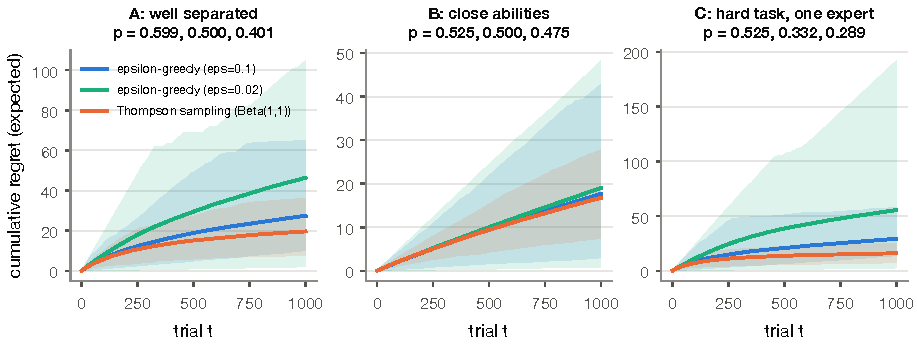
\includegraphics[width=\textwidth]{figures/fig_q1_regret.pdf}
\caption{Cumulative expected regret over 1000 trials (mean over 200 runs, shaded 10--90\% range) for the three settings of Table~\ref{tab:q1}.}
\label{fig:q1}
\end{figure}

\emph{Effect of the gap between arms.} The gap between the best and the second-best member determines both how fast an algorithm can identify the best arm and how much each mistake costs. With a clear gap (A: 0.10; C: 0.19) Thompson sampling identifies the expert within a few hundred trials and its regret curve flattens (19.6 and 16.1 after 1000 trials, about 3\% of the oracle reward); $\epsilon$-greedy with $\epsilon=0.1$ also finds the best arm quickly but keeps paying $\approx\epsilon T\bar\Delta$ for its constant exploration, so its regret grows linearly (27--29); with $\epsilon=0.02$ exploration is too rare to correct early unlucky estimates, which produces the widest spread of outcomes (10--90\% range up to 192 in C) and the worst mean. With a tiny gap (B: 0.025) no algorithm can separate the arms within 1000 trials, the posteriors of Thompson sampling stay overlapping and it keeps exploring, yet the regret is small (17--19) because the arms are nearly equivalent: a small gap slows learning but also makes learning less important. Thompson sampling is the best or tied-best in every setting because its exploration adapts to the evidence, whereas $\epsilon$-greedy's exploration rate must be tuned per problem.

\subsection{Q2 Contextual bandit for task assignment}
\subsubsection{Q2.a Algorithm} Each round presents three tasks (types $j=1,2,3$, difficulties $\delta_j$) and the agent chooses a one-to-one assignment $\sigma$ (member $i$ gets task $\sigma(i)$); the reward is the number of completed tasks, $\sum_i X_i$ with $X_i\sim\text{Bernoulli}(p_{i\sigma(i)})$, $p_{ij}=\sigma(\beta_{ij}-\delta_j)$. We implemented \emph{combinatorial Thompson sampling} \cite{gai2012,wang2018}: (i) keep an independent Beta$(a_{ij},b_{ij})$ posterior for each of the nine member-task pairs (starting from Beta$(1,1)$), which is sufficient because the expected reward of an assignment is the sum of its pair probabilities; (ii) each round draw one sample $\tilde p_{ij}$ from every posterior and choose the assignment maximising $\sum_i\tilde p_{i\sigma(i)}$, a maximum-weight bipartite matching (we enumerate the $3!=6$ permutations; the Hungarian algorithm would be used for larger teams); (iii) observe the three outcomes and update the three posteriors that were used (semi-bandit feedback). Sampling makes an uncertain pair occasionally look good enough to be tried (exploration) while pairs with concentrated posteriors are assigned according to their means (exploitation); the amount of exploration shrinks automatically as posteriors narrow. The learned success probabilities map to abilities through $\hat\beta_{ij}=\text{logit}(\hat p_{ij})+\delta_j$ when the difficulties are known. As a baseline we use $\epsilon$-greedy matching ($\epsilon=0.1$): the assignment maximising the sample means, or a random permutation with probability $\epsilon$.

\subsubsection{Q2.b Simulation and analysis} Three settings vary the diversity of abilities across task types (Table~\ref{tab:q2}): specialists (each member is good at one task type), generalists (all members similar, small differences) and one strong member. Results over 200 runs of $T=1000$ rounds are compared with the oracle that always uses the optimal assignment (Fig.~\ref{fig:q2}); Fig.~\ref{fig:q2learned} shows the true and the learned success matrices of one run.

\begin{table}[t]
\centering\scriptsize
\caption{Q2.b: settings and results (200 runs of 1000 rounds). ``Gap'' is the expected-reward difference between the best and the second-best assignment; ``opt.\ end'' is the share of runs whose last assignment is the optimal one; reward is agent/oracle over 1000 rounds.}
\label{tab:q2}
\setlength{\tabcolsep}{2pt}
\begin{tabular}{l>{\raggedright\arraybackslash}p{3.1cm}lcc|ccc|ccc}
\toprule
 & & & & & \multicolumn{3}{c|}{combinatorial Thompson} & \multicolumn{3}{c}{$\epsilon$-greedy matching}\\
Setting & $\beta_{ij}$ (rows: members) & $\delta_j$ & oracle/round & gap & regret & reward & opt.\ end & regret & reward & opt.\ end\\
\midrule
A specialists & diagonal 0.9, others 0.1 & 0.5/0.5/0.5 & 1.796 & 0.395 & \textbf{29.1} & 1771/1796 & 0.97 & 59.9 & 1732/1796 & 0.91\\
B generalists & $0.5\pm0.05$ & 0.3/0.5/0.7 & 1.537 & 0.025 & \textbf{26.3} & 1512/1537 & 0.34 & 27.1 & 1508/1537 & 0.35\\
C one strong member & member 1: 1.0/0.9/0.8; others $\le0.7$ & 0.4/0.6/0.8 & 1.621 & 0.096 & \textbf{45.3} & 1572/1621 & 0.86 & 59.0 & 1561/1621 & 0.69\\
\bottomrule
\end{tabular}
\end{table}

\begin{figure}[t]
\centering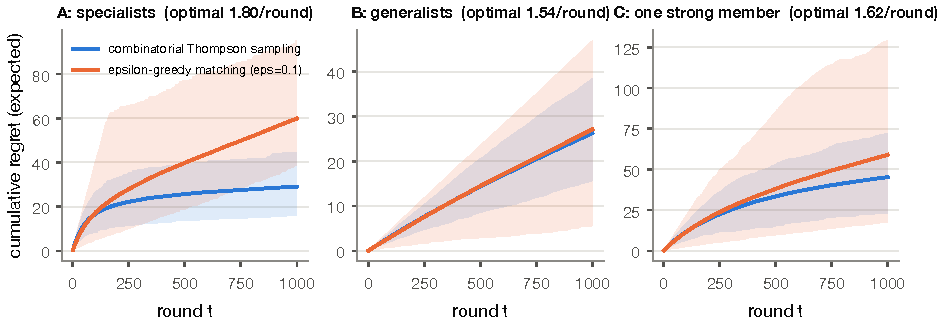
\includegraphics[width=\textwidth]{figures/fig_q2_regret.pdf}
\caption{Cumulative expected regret of the assignment algorithms (mean over 200 runs, 10--90\% band).}
\label{fig:q2}
\end{figure}
\begin{figure}[t]
\centering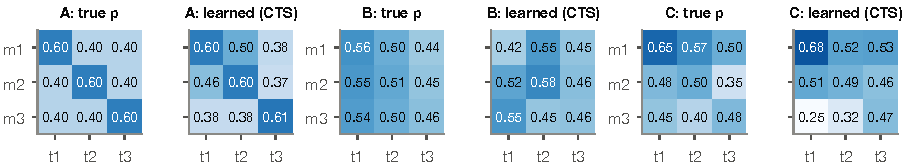
\includegraphics[width=\textwidth]{figures/fig_q2_learned.pdf}
\caption{True success probabilities $p_{ij}$ and the posterior means learned by combinatorial Thompson sampling after 1000 rounds (one run per setting; rows: members, columns: task types).}
\label{fig:q2learned}
\end{figure}

\emph{Effect of ability diversity.} When abilities are diverse across task types (A), the optimal assignment is worth 0.40 more tasks per round than the runner-up, so the evidence for it accumulates fast: the Thompson matcher's regret rises to 21 in the first 200 rounds and only to 29 after 1000 (1.6\% of the oracle's reward), and 97\% of the runs end on the optimal assignment. When members are interchangeable (B) the best assignment is only 0.025 tasks per round better than the second best; the algorithm cannot resolve the ordering within 1000 rounds (34\% end optimal) and its regret grows almost linearly, but the total loss stays tiny (1.7\%) because any assignment is nearly as good. The mixed setting (C) is the slowest: the strong member is placed correctly early, but ordering the two weaker members on the remaining tasks involves pairs that differ by less than 0.1, so the regret keeps growing (45) and 86\% of runs end optimal. Diversity therefore speeds up learning and raises the value of learning at the same time; the learned matrices are accurate for the pairs on the optimal assignment and remain rough for pairs that are rarely tried (e.g.\ member 3 in setting C), which is exactly what a decision-focused learner should do. Thompson sampling beats $\epsilon$-greedy matching by a factor of two in A and C and ties in B, for the same reason as in Q1.

\subsection{Q3 Bayesian reinforcement learning}
\subsubsection{Q3.a MDP simulation and data collection} The simulator implements the transition table and the reward model ($r=0$ for \code{rest}, $r\sim\mathcal N(\mu_s,0.3)$ with $\mu=(1.0,0.5,-0.5)$ for \code{work}). One trajectory of 100 steps from $s_0=\text{fresh}$ under the random policy ($P(\text{work})=0.5$) visited fresh/tired/exhausted 40/35/25 times; the state-action counts were fresh: 21 rest, 19 work; tired: 15 rest, 20 work; exhausted: 14 rest, 11 work (Fig.~\ref{fig:q3}a). Observed transition counts $(s'\!=\!\text{fresh},\text{tired},\text{exhausted})$: fresh/rest (20,1,0), fresh/work (8,10,1), tired/rest (9,6,0), tired/work (0,8,12), exhausted/rest (2,10,2), exhausted/work (0,0,11). Rewards: the 50 rest steps gave exactly 0; the work rewards had mean 0.96 (sd 0.28, $n{=}19$) when fresh, 0.43 (sd 0.36, $n{=}20$) when tired and $-0.43$ (sd 0.32, $n{=}11$) when exhausted; the total return of the random policy was 22.1 (0.22 per step).

\subsubsection{Q3.b Bayesian inference of the MDP parameters} We used the suggested model, $\theta_{s,a}\sim\text{Dirichlet}(1,1,1)$, $s'\sim\text{Categorical}(\theta_{s,a})$ for all six pairs, and $\mu_{s}\sim\mathcal N(0,2)$, $\sigma_{s}\sim\text{HalfNormal}(2)$, $r\sim\mathcal N(\mu_s,\sigma_s)$ for the three \emph{work} pairs. The reward of \code{rest} is zero by construction (no task is attempted), so $E[r\mid s,\text{rest}]=0$ is treated as known: fitting the Normal model to 50 observations that are all exactly 0 would make the posterior of $\sigma_{s,\text{rest}}$ degenerate (unbounded density at 0) and the sampler unstable. NUTS (4 chains $\times$ 1500 draws) converged cleanly ($\Rhat\le1.001$, ESS $\ge4570$, no divergences). Table~\ref{tab:q3} compares the posterior means with the truth; the transition posteriors coincide with the conjugate Dirichlet update $(1+n_{s,a,s'})/(3+n_{s,a})$ to three decimals, which validates the implementation.

\begin{table}[t]
\centering\footnotesize
\caption{Q3.b: true parameters versus posterior means (95\% HDI in brackets for the reward means and the largest-error transition of each pair).}
\label{tab:q3}
\setlength{\tabcolsep}{3pt}
\begin{tabular}{ll cc cc cc c}
\toprule
 & & \multicolumn{2}{c}{$P(s'{=}\text{fresh}\mid s,a)$} & \multicolumn{2}{c}{$P(s'{=}\text{tired}\mid s,a)$} & \multicolumn{2}{c}{$P(s'{=}\text{exhausted}\mid s,a)$} & $E[r\mid s,a]$\\
$s$ & $a$ ($n$) & true & posterior & true & posterior & true & posterior & true / posterior\\
\midrule
fresh & rest (21) & 0.9 & 0.875 \HDI{0.74}{0.98} & 0.1 & 0.083 & 0.0 & 0.042 & 0 / 0 (known)\\
fresh & work (19) & 0.3 & 0.408 \HDI{0.21}{0.61} & 0.6 & 0.501 & 0.1 & 0.091 & 1.0 / 0.96 \HDI{0.82}{1.09}\\
tired & rest (15) & 0.6 & 0.557 \HDI{0.34}{0.78} & 0.4 & 0.388 & 0.0 & 0.055 & 0 / 0 (known)\\
tired & work (20) & 0.0 & 0.044 & 0.4 & 0.393 & 0.6 & 0.563 \HDI{0.37}{0.76} & 0.5 / 0.43 \HDI{0.27}{0.61}\\
exhausted & rest (14) & 0.2 & 0.177 & 0.7 & 0.648 \HDI{0.43}{0.86} & 0.1 & 0.175 & 0 / 0 (known)\\
exhausted & work (11) & 0.0 & 0.071 & 0.1 & 0.070 & 0.9 & 0.859 \HDI{0.68}{1.00} & $-0.5$ / $-0.43$ \HDI{-0.67}{-0.22}\\
\bottomrule
\end{tabular}
\end{table}

\begin{figure}[t]
\centering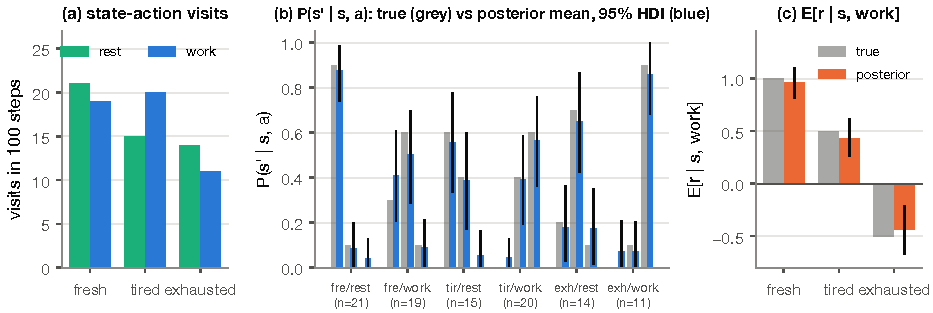
\includegraphics[width=\textwidth]{figures/fig_q3.pdf}
\caption{Q3: (a) state-action visits of the 100-step random-policy trajectory; (b) true transition probabilities (grey) versus posterior means with 95\% HDIs (blue); the three bars of each state-action pair are $s'=$ fresh, tired, exhausted; (c) true versus posterior work-reward means.}
\label{fig:q3}
\end{figure}

\emph{Accuracy.} Every true value lies inside its 95\% HDI. The mean absolute error of the 18 transition probabilities is 0.044 (maximum 0.108 for $P(\text{fresh}\mid\text{fresh},\text{work})$, estimated 0.41 from 19 visits), the reward means are within 0.07 of the truth, and the reward noise is recovered (0.30, 0.39, 0.37 versus 0.3). Two systematic effects are visible: transitions that are impossible in the true MDP receive 4--7\% posterior mass because the flat Dirichlet prior adds one pseudo-count per successor, and the pairs visited least (exhausted/work, 11 visits) have the widest intervals. \emph{Improvements:} (i) more data, since interval widths shrink with $1/\sqrt{n_{s,a}}$; (ii) an exploration policy that targets under-visited pairs instead of choosing at random, e.g.\ count-based exploration or posterior sampling over MDPs (PSRL \cite{osband2013}), which also earns reward while learning; (iii) weakly informative priors that use structure, such as a smaller concentration for transitions that skip a fatigue level or the knowledge that fatigue changes by at most one level per step; (iv) sharing information across states (e.g.\ a monotone effect of fatigue on the reward mean) and, as done here, treating known quantities such as the zero rest reward as fixed.

\subsubsection{Q3.c Policy optimisation} With the posterior-mean parameters $\hat P$, $\hat\mu$ we solved $\min\sum_s v(s)$ s.t.\ $v(s)\ge R(s,a)+\gamma\sum_{s'}\hat P(s'\mid s,a)v(s')$ for all $(s,a)$ (Pyomo/HiGHS), where $R(s,\text{work})=\hat\mu_s$ and $R(s,\text{rest})=0$; the horizon is infinite, so a discount factor is needed and we report $\gamma=0.9$ (0.95 and 0.99 give the same policy). The optimal policy is
\begin{equation*}
\pi^\ast(\text{fresh})=\text{work},\quad \pi^\ast(\text{tired})=\text{rest},\quad \pi^\ast(\text{exhausted})=\text{rest};\qquad
V^\ast=(4.87,\;4.04,\;3.71),
\end{equation*}
with $Q(\text{fresh},\cdot)=(4.28,4.87)$, $Q(\text{tired},\cdot)=(4.04,3.93)$ and $Q(\text{exhausted},\cdot)=(3.71,3.00)$ for (rest, work). The LP on the \emph{true} parameters yields the same policy with $V^\ast=(4.90,4.14,3.83)$, and evaluating the learned policy on the true MDP gives exactly these values, i.e.\ the model error costs nothing in this case. The policy makes intuitive sense: working when fresh earns the +1 reward and usually leads to tiredness, which resting repairs quickly (60\% back to fresh) at no cost; working when tired earns only 0.5 and, with probability 0.6, leads to exhaustion, where work is punished ($-0.5$) and recovery is slow, so the agent rests; when exhausted, resting is clearly better than working. The decision at \emph{tired} is a close call ($Q$ values 4.04 versus 3.93), which is why the accuracy of the learned transition probabilities matters and why a decision maker should keep track of the posterior uncertainty (for example by solving the LP for several posterior draws) before deploying such a policy.

\clearpage
\begin{thebibliography}{99}\small
\bibitem{cortez2008} P.\ Cortez and A.\ Silva. Using data mining to predict secondary school student performance. In \emph{Proceedings of the 5th Future Business Technology Conference (FUBUTEC 2008)}, pages 5--12. EUROSIS, 2008.
\bibitem{sirin2005} S.\ R.\ Sirin. Socioeconomic status and academic achievement: A meta-analytic review of research. \emph{Review of Educational Research}, 75(3):417--453, 2005.
\bibitem{coleman1966} J.\ S.\ Coleman et al. \emph{Equality of Educational Opportunity}. U.S.\ Government Printing Office, Washington, DC, 1966.
\bibitem{raudenbush2002} S.\ W.\ Raudenbush and A.\ S.\ Bryk. \emph{Hierarchical Linear Models: Applications and Data Analysis Methods}, 2nd edition. Sage, 2002.
\bibitem{gelman2020} A.\ Gelman, A.\ Vehtari, D.\ Simpson, C.\ C.\ Margossian, B.\ Carpenter, Y.\ Yao, L.\ Kennedy, J.\ Gabry, P.-C.\ B\"urkner, and M.\ Modr\'ak. Bayesian workflow. \emph{arXiv:2011.01808}, 2020.
\bibitem{vehtari2017} A.\ Vehtari, A.\ Gelman, and J.\ Gabry. Practical Bayesian model evaluation using leave-one-out cross-validation and WAIC. \emph{Statistics and Computing}, 27:1413--1432, 2017.
\bibitem{kwiatkowska2011} M.\ Kwiatkowska, G.\ Norman, and D.\ Parker. PRISM 4.0: Verification of probabilistic real-time systems. In \emph{Proc.\ CAV 2011}, LNCS 6806, pages 585--591. Springer, 2011.
\bibitem{kochenderfer2022} M.\ J.\ Kochenderfer, T.\ A.\ Wheeler, and K.\ H.\ Wray. \emph{Algorithms for Decision Making}. MIT Press, 2022.
\bibitem{lattimore2020} T.\ Lattimore and C.\ Szepesv\'ari. \emph{Bandit Algorithms}. Cambridge University Press, 2020.
\bibitem{rasch1960} G.\ Rasch. \emph{Probabilistic Models for Some Intelligence and Attainment Tests}. Danish Institute for Educational Research, Copenhagen, 1960.
\bibitem{gai2012} Y.\ Gai, B.\ Krishnamachari, and R.\ Jain. Combinatorial network optimization with unknown variables: Multi-armed bandits with linear rewards and individual observations. \emph{IEEE/ACM Transactions on Networking}, 20(5):1466--1478, 2012.
\bibitem{wang2018} S.\ Wang and W.\ Chen. Thompson sampling for combinatorial semi-bandits. In \emph{Proc.\ ICML 2018}, PMLR 80, pages 5114--5122, 2018.
\bibitem{osband2013} I.\ Osband, D.\ Russo, and B.\ Van Roy. (More) efficient reinforcement learning via posterior sampling. In \emph{Advances in Neural Information Processing Systems 26}, 2013.
\end{thebibliography}

\end{document}
